%===============================================================================
\section{La causalidad y la noción de ceteris paribus en el análisis econométrico}
%===============================================================================

%-------------------------------------------------------------------------------
\subsection{Coeficiente de correlación}
%-------------------------------------------------------------------------------
\begin{frame}{Coeficiente de correlación}
	\begin{itemize}
		\item Mide la asociación lineal entre dos variables.
		\item Poblacionalmente la covarianza se mide como:
		$$Cov(y,x)=E[(y-E(y))(x-E(x))]$$
		\item Muestralmente se estima como:
		$$\sigma_{y,x}=\frac{\sum_{i=1}^T(x_i-\bar{x})(y_i-\bar{y})}{T-1}$$
		\item Correlación muestral
		$$\rho_{y,x}=\frac{\sigma_{y,x}}{\sigma_{y}\sigma_{x}}$$
	\end{itemize}
\end{frame}
%------------------------------------------------
\begin{frame}{Coeficiente de correlación}
	\begin{figure}
		\centering
		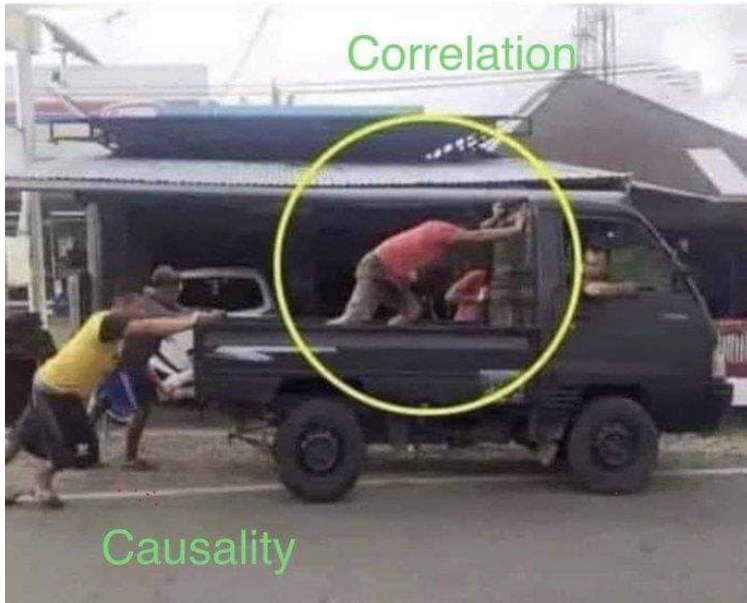
\includegraphics[scale=.36]{figuras/cau_y_corr_1.png}
	\end{figure}
\end{frame}
%------------------------------------------------
\begin{frame}{Coeficiente de correlación}
	\begin{figure}
		\centering
		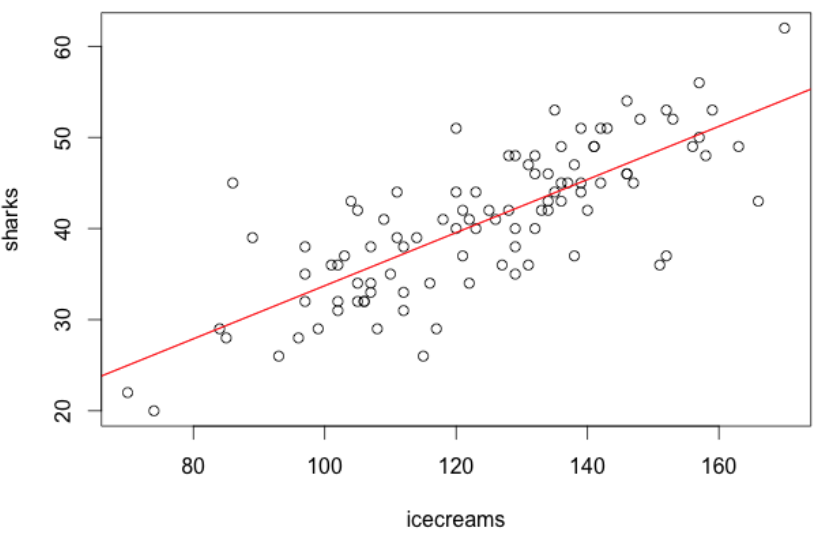
\includegraphics[scale=.36]{figuras/cau_y_corr_2.png}
	\end{figure}
\end{frame}